\documentclass[11pt,a4paper]{article}

\usepackage[T1]{fontenc}
\usepackage[utf8]{inputenc}
\usepackage{lmodern}
\usepackage{microtype}
\usepackage{geometry}
\usepackage{amsmath,amssymb}
\usepackage{booktabs}
\usepackage{graphicx}
\usepackage{hyperref}
\usepackage[numbers,sort&compress]{natbib}

\geometry{margin=2.45cm}
\graphicspath{{generated/}{../generated/}}
\hypersetup{colorlinks=true,linkcolor=blue!55!black,citecolor=blue!55!black,urlcolor=blue!55!black}
\newcommand{\Mpl}{M_{\rm Pl}}
\newcommand{\repo}{\href{https://github.com/MartinPetrasek123/MartinPetrasek123/tree/main/r-universe-global-kgb-completion}{public reproducibility package}}

\title{\textbf{R-Universe: A Global Luminal Kinetic-Gravity-Braiding Completion of the R$\alpha$ Background}}
\author{Martin Petr\'a\v{s}ek\\
\small Institute for Resonant Synthesis and Field Physics, Prague, Czech Republic}
\date{Technical completion note, 9 August 2026}

\begin{document}
\maketitle

\begin{abstract}
The R$\alpha$ R-Universe branch fits a finite-window late-time background but, by itself, does not define a covariant perturbation theory. This note gives one explicit covariant completion. The action is a luminal kinetic-gravity-braiding (KGB) theory with constant Planck mass and minimally coupled matter. It reproduces the fitted R$\alpha$ background exactly on the entire observed past light cone, smoothly completes the previously unspecified future to a de Sitter branch, and specifies the action functions $A(\phi)$, $B(\phi)$, $C(\phi)$ and $V(\phi)$ for every scalar-field value. The scalar no-ghost discriminant, scalar gradient numerator, tensor kinetic coefficient and tensor speed are positive on $10^{-8}\le a\le10^3$; the construction sets $c_s^2=1$. A native H--EFTCAMB run evolves the photon--baryon--CDM--neutrino--KGB system, and its CMB plus lensing spectra are evaluated at one declared point with the official Planck 2018 likelihoods. This is a fixed-point calculation, not a posterior, model comparison, or replacement claim for $\Lambda$CDM.
\end{abstract}

\section{Defined theory}

The covariant action is
\begin{equation}
S=\int d^4x\sqrt{-g}\left[\frac{\Mpl^2}{2}R+A(\phi)X+B(\phi)X^2-V(\phi)-C(\phi)X\Box\phi\right]+S_m[g,\psi_m],
\qquad X\equiv-\frac12(\nabla\phi)^2.
\label{eq:action}
\end{equation}
It is the $G_2+G_3$ luminal Horndeski/KGB subclass \citep{Deffayet2010}.  This
class has the standard constrained scalar--tensor field content, rather than
the higher-derivative mode of a generic $\Box\phi$ theory. The constant coefficient of $R$ gives
\begin{equation}
Q_T=\Mpl^2,\qquad c_T^2=1,\qquad d_L^{\rm GW}/d_L^{\rm EM}=1.
\label{eq:tensor}
\end{equation}
The action is defined off shell by taking $\phi/\Mpl=\ln a$ as the field coordinate used to specify its functions; this is not a restriction of inhomogeneous field configurations. For any $\phi$, the unique expanding background root defines $E(\phi)$ and therefore $A(\phi)$, $B(\phi)$, $C(\phi)$ and $V(\phi)$. The exact definitions and source code are in \repo.

\section{Global R$\alpha$ background}

For all observed epochs, $a\le1$, the background is exactly the fitted R$\alpha$ relation
\begin{equation}
E^2=\Omega_{\rm m0}a^{-3}+\Omega_{\rm r0}a^{-4}+r,
\qquad r=\Omega_{\mathcal R0}E^{\alpha a}.
\label{eq:observed-background}
\end{equation}
Thus no late-time likelihood datum is altered by the completion. To define the theory globally, $a$ in the exponent is replaced only for $a>1$ by a $C^\infty$ function $a_{\rm eff}(a)$ that equals $a$ for $a\le1$ and equals two for $a\ge2$. The global response is
\begin{equation}
r=\Omega_{\mathcal R0}E^{\alpha a_{\rm eff}(a)}.
\label{eq:global-background}
\end{equation}
For $\alpha<1$, it has the unique future de Sitter limit
\begin{equation}
E_\infty=\Omega_{\mathcal R0}^{1/(2-2\alpha)}.
\end{equation}

With $N=\ln a$, $x=\alpha a_{\rm eff}$, the derivatives used in the reconstruction are
\begin{equation}
E_N=\frac{rx_N\ln E-3\Omega_{\rm m0}a^{-3}-4\Omega_{\rm r0}a^{-4}}{2E-rx/E},
\qquad r_N=r\left(x_N\ln E+x\frac{E_N}{E}\right).
\label{eq:background-derivatives}
\end{equation}

\section{Scalar completion and stability}

The regular radiation-limit closure is
\begin{equation}
\alpha_B=\frac{\Omega_{\mathcal R}}{3},\qquad
\alpha_{B,N}=\frac{\Omega_{\mathcal R,N}}{3}.
\label{eq:alphaB}
\end{equation}
In radiation domination, $\Omega_{\mathcal R,N}\to4\Omega_{\mathcal R}$ and $-E_N/E\to2$, giving $D/\Omega_{\mathcal R}\to1$. Thus the scalar kinetic sector decouples with the R-sector energy fraction and the coefficient $1/3$ is fixed without a new sampled parameter.

For $\alpha_M=\alpha_T=0$, the scalar conditions in the Bellini--Sawicki convention \citep{BelliniSawicki2014} are
\begin{align}
D&=\alpha_K+\frac32\alpha_B^2,\qquad
Q_s=\frac{2\Mpl^2D}{(2-\alpha_B)^2},\\
\mathcal N_s&=(2-\alpha_B)\left(-\frac{E_N}{E}+\frac{\alpha_B}{2}\right)+\alpha_{B,N}-(3\Omega_m+4\Omega_r),
\qquad c_s^2=\frac{\mathcal N_s}{D}.
\label{eq:scalar-stability}
\end{align}
The closure prescription is
\begin{equation}
D=\mathcal N_s,\qquad \alpha_K=D-\frac32\alpha_B^2,
\label{eq:closure}
\end{equation}
which gives $c_s^2=1$ identically after the independently checked condition $\mathcal N_s>0$.

Set $X=E^2/2$, $C=\alpha_B/E^2$, and define
\begin{align}
\rho_\phi&=3r,&p_\phi&=-3r-r_N,\\
R_\rho&=\rho_\phi-6E^2XC+2C_\phi X^2,&
R_p&=p_\phi+2C_\phi X^2+2CXEE_N.
\end{align}
Then the action functions are
\begin{align}
B&=\frac{\alpha_KE^2-(R_\rho+R_p)+8C_\phi X^2-12E^2XC}{8X^2},\\
A&=\frac{R_\rho+R_p-4BX^2}{2X},\qquad
V=\frac{R_\rho-R_p}{2}-BX^2.
\label{eq:reconstruction}
\end{align}
Direct substitution in the KGB density and pressure equations reproduces $\rho_\phi$ and $p_\phi$. The source package checks the reconstruction at 80-digit precision where radiation-era cancellations exceed binary64 resolution.

At the distance-fit point $(\Omega_{\rm m0},\Omega_{\rm r0},\alpha)=(0.3022734375,9.083909\times10^{-5},0.497421875)$, the full-domain checks give
\begin{equation}
\min\mathcal N_s=7.680\times10^{-29},\quad
\min D=7.680\times10^{-29},\quad
\min(Q_s/\Mpl^2)=3.840\times10^{-29},\quad
\max|c_s^2-1|=0.
\end{equation}
The background residual is below $6.2\times10^{-16}$ and the high-precision action reconstruction residual is below $1.8\times10^{-81}$.

\begin{figure}[htbp]
\centering
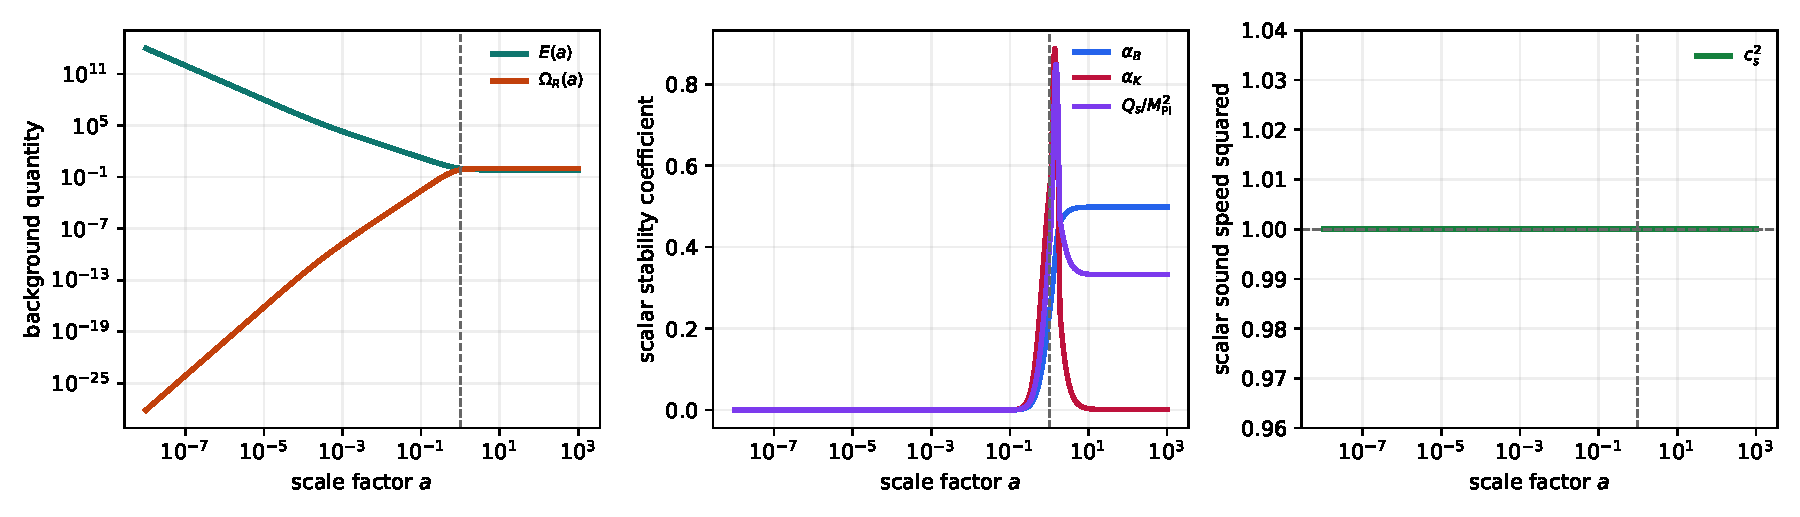
\includegraphics[width=\linewidth]{ru_kgb_stability.pdf}
\caption{Global R$\alpha$ KGB completion. The first panel shows the background solution and R-sector fraction; the second shows the action-derived scalar coefficients; the third verifies $c_s^2=1$. The dashed line is $a=1$, the end of the observationally fitted interval and the start of the smooth future completion.}
\label{fig:stability}
\end{figure}

\section{Matter, early universe, and local gravity}

The action fixes the high-wavenumber quasistatic response rather than assigning an independent phenomenological function:
\begin{equation}
\mu_\infty=1+\frac{\alpha_B^2}{2Dc_s^2},\qquad
\eta_\infty=1,\qquad\Sigma_\infty=\mu_\infty.
\label{eq:mu}
\end{equation}
Integrating the corresponding matter-growth equation gives $1\le\mu_\infty\le1.05877$ and $D_+/D_{+,\Lambda{\rm CDM}}\in[0.99939,1.01047]$ over $10^{-3}\le a\le1$ for the stated same-parameter comparison.

At recombination, the R-sector fraction is $1.345\times10^{-9}$, the relative background expansion shift is $3.07\times10^{-12}$, and the action-derived high-$k$ scalar response is $\mu_\infty-1=3.62\times10^{-5}$. A direct background sound-horizon integral with the declared baryon input gives $r_s=147.8939533\,{\rm Mpc}$ and differs from the same-parameter $\Lambda$CDM background by $-4.90\times10^{-13}$. This is a necessary early-universe gate; it is not a $C_\ell$ likelihood.

The cubic KGB coefficient implies $\Lambda_3^3=\Mpl H_0^2/|\hat C_0|$. Matching Eq.~\eqref{eq:mu} to $2\beta_{\rm eff}^2=\mu_\infty-1$ gives $\beta_{\rm eff}=0.17142$. The decoupling-limit Vainshtein scale of a Solar-mass source is $r_V=97.81\,{\rm pc}$. At a Cassini impact parameter $1.6R_\odot$, the conservative screened envelope is $|\gamma-1|\le8.33\times10^{-16}$, below $2.3\times10^{-5}$ \citep{Bertotti2003}. This is an analytic screening gate of Eq.~\eqref{eq:action}, not an ephemeris re-fit.

\section{Native CMB calculation and claim boundary}

The exact $w_R(a)$, $\alpha_K(a)$, and $\alpha_B(a)$ functions are passed to
the H--EFTCAMB reparametrized-Horndeski interface, with the explicit convention
$\alpha_B^{\rm RPH}=-\alpha_B^{\rm BS}/2$. The native run evolves photons,
baryons, CDM, three massless neutrinos, metric constraints, and the KGB scalar.
At the fixed inputs $\omega_b=0.02237$, $A_s=2.1\times10^{-9}$,
$n_s=0.9649$, $\tau=0.0544$, and $A_{\rm Planck}=1$, the action fixes
$H_0=67.86230797\,{\rm km\,s^{-1}\,Mpc^{-1}}$ and $\omega_c=0.116836$.
The official Planck 2018 Plik-lite TTTEEE, Commander TT, SimAll EE, and
CMB-dependent lensing likelihood objects \citep{Planck2018V} give
\begin{equation}
-2\ln\mathcal L_{\rm Planck}=1210.1599180.
\end{equation}
The 201-to-601-node spline change is $8.84\times10^{-6}$ in this value; the
change induced by moving the numerical perturbation turn-on from $10^{-4}$ to
$10^{-3}$ is $-2.94\times10^{-5}$. The source and machine-readable reports
are in \repo. This absolute likelihood includes normalization terms and is not
a goodness-of-fit $\chi^2$.

\section{Reproducibility and claim boundary}

All equations, precision checks, parameter scan, source table, figure, matter prediction, early-universe gate, and PPN screening calculation are regenerated by
\begin{verbatim}
bash scripts/run_all.sh
\end{verbatim}
in \repo. The Planck fixed-point evaluation additionally uses the official Planck distribution and the H--EFTCAMB executable. A statement that R-Universe replaces $\Lambda$CDM requires a joint parameter posterior, BAO, supernova, RSD, matter-lensing, and local-gravity inference, followed by a declared model comparison. This technical note does not predeclare that outcome.

The independent action-identity validation additionally recomputes $E_N$,
$r_N$, $\alpha_B$, $\alpha_K$, and the homogeneous scalar equation from the
declared $G_2+G_3$ action. Its report is part of the source package.

\begin{thebibliography}{9}
\bibitem[Deffayet et al.(2010)]{Deffayet2010}
C. Deffayet, O. Pujol\`as, I. Sawicki and A. Vikman, ``Imperfect Dark Energy from Kinetic Gravity Braiding,'' \emph{JCAP} 10 (2010) 026, \href{https://arxiv.org/abs/1008.0048}{arXiv:1008.0048}.
\bibitem[Bellini \& Sawicki(2014)]{BelliniSawicki2014}
E. Bellini and I. Sawicki, ``Maximal freedom at minimum cost: linear large-scale structure in general modifications of gravity,'' \emph{JCAP} 07 (2014) 050, \href{https://doi.org/10.1088/1475-7516/2014/07/050}{doi:10.1088/1475-7516/2014/07/050}.
\bibitem[Bertotti et al.(2003)]{Bertotti2003}
B. Bertotti, L. Iess and P. Tortora, ``A test of general relativity using radio links with the Cassini spacecraft,'' \emph{Nature} 425 (2003) 374--376, \href{https://doi.org/10.1038/nature01997}{doi:10.1038/nature01997}.
\bibitem[Planck Collaboration(2020)]{Planck2018V}
Planck Collaboration, ``Planck 2018 results. V. CMB power spectra and likelihoods,'' \emph{Astronomy \& Astrophysics} 641 (2020) A5, \href{https://arxiv.org/abs/1907.12875}{arXiv:1907.12875}.
\end{thebibliography}

\end{document}
